\documentclass{standalone}
\usepackage{tikz}
\usepackage{amsmath}
\usetikzlibrary{arrows.meta, positioning}

\begin{document}
	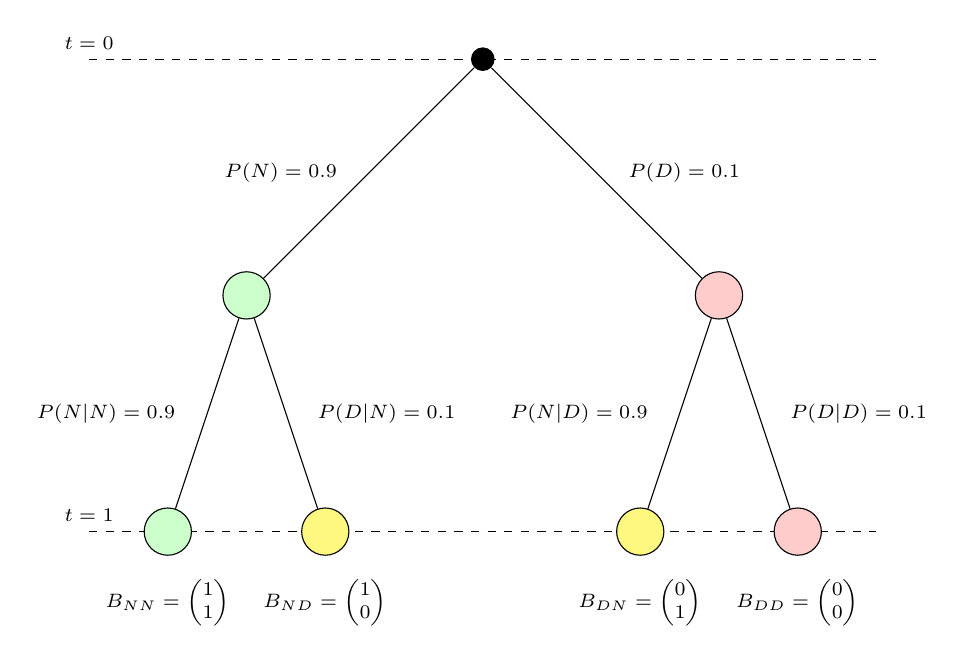
\begin{tikzpicture}[
		every node/.style={font=\scriptsize, align=center},
		edge from parent/.style={draw, -{Stealth}},
		level distance=30mm,
		sibling distance=30mm
		]
		
		% Dashed line for t=0
		\draw[dashed] (-5, 0) -- (5, 0);
		\node[above] at (-5, 0) {$t = 0$};
		
		% Initial node at t=0
		\node[fill=black, circle, minimum size=3mm, inner sep=0pt] (A) at (0, 0) {};
		
		% Nodes at t=1
		\node[fill=green!20, draw=black, circle, minimum size=6mm, inner sep=0pt] (B1) at (-3, -3) {};
		\node[fill=red!20, draw=black, circle, minimum size=6mm, inner sep=0pt] (B2) at (3, -3) {};
		
		% Edges and edge labels from t=0 to t=1
		\draw (A) -- (B1) node[midway, left=8pt] {$P(N) = 0.9$};
		\draw (A) -- (B2) node[midway, right=8pt] {$P(D) = 0.1$};
		
		% Dashed line for t=1
		\draw[dashed] (-5, -6) -- (5, -6);
		\node[above] at (-5, -6) {$t = 1$};
		
		% Nodes at t=1 (bottom layer)
		\node[fill=green!20, draw=black, circle, minimum size=6mm, inner sep=0pt] (C1) at (-4, -6) {}; % Both non-default
		\node[fill=yellow!50, draw=black, circle, minimum size=6mm, inner sep=0pt] (C2) at (-2, -6) {}; % One default (N-D)
		\node[fill=yellow!50, draw=black, circle, minimum size=6mm, inner sep=0pt] (C3) at (2, -6) {};  % One default (D-N)
		\node[fill=red!20, draw=black, circle, minimum size=6mm, inner sep=0pt] (C4) at (4, -6) {};  % Both default
		
		% Edges and edge labels from t=1 to t=1 (bottom layer)
		\draw (B1) -- (C1) node[midway, left=8pt] {$P(N|N) = 0.9$};
		\draw (B1) -- (C2) node[midway, right=8pt] {$P(D|N) = 0.1$};
		\draw (B2) -- (C3) node[midway, left=8pt] {$P(N|D) = 0.9$};
		\draw (B2) -- (C4) node[midway, right=8pt] {$P(D|D) = 0.1$};
		
		% Payoffs below the nodes at t=1
		\node[below=5pt] at (C1.south) {$B_{NN} = \begin{pmatrix} 1 \\ 1 \end{pmatrix}$};
		\node[below=5pt] at (C2.south) {$B_{ND} = \begin{pmatrix} 1 \\ 0 \end{pmatrix}$};
		\node[below=5pt] at (C3.south) {$B_{DN} = \begin{pmatrix} 0 \\ 1 \end{pmatrix}$};
		\node[below=5pt] at (C4.south) {$B_{DD} = \begin{pmatrix} 0 \\ 0 \end{pmatrix}$};
		
	\end{tikzpicture}
\end{document}
